\def\classe{\textsf{PSI $\star$}}
%\def\classe{\textsf{MP}}
%\def\classe{\textsf{MPSI}}
\def\xxnumpartie{}
\def\xxpartie{}%Modéliser et corriger le comportement linéaire et non linéaire des systèmes multiphysiques}
\def\xxnumchapitre{Devoir surveillé 2 \vspace{.2cm}}
\def\xxchapitre{\hspace{.12cm} }
%\def\discipline{Informatique}
\def\discipline{Sciences \\ Industrielles \\de l'Ingénieur}
\def\xxtete{\discipline}
\def\xxactivite{\textsf{DS 2}}
\def\xxonglet{\textsf{\xxactivite}}
\def\xxauteur{\textsl{Xavier Pessoles}}

\def\xxtitreexo{\noindent  }
\def\xxsourceexo{\hspace{.2cm}}


\def\xxfigures{}%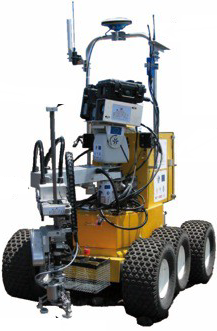
\includegraphics[width=.5\linewidth]{fig_00}}
\def\xxpied{%
\textsf{\xxactivite}%dans le but de déterminer les contraintes géométriques dans les mécanismes\\% afin de valider leurs performances.\\
%Révisions 1 -- 2 -- 3 -- \xxactivite%
}

\def\xxposongletx{2}
\def\xxposonglettext{1.45}
\def\xxposonglety{20}
%\def\xxonglet{Part. 1 -- Ch. 3}

